%--- Analisi dei requisiti ---------------------------------------------------
\chapter{Analisi dei requisiti}
\label{chap:analisi-requisiti}

\section{Casi d'uso}
Per lo studio dei casi di utilizzo del prodotto sono stati creati dei diagrammi.
I diagrammi dei casi d'uso sono diagrammi di tipo \gls{uml} dedicati alla descrizione delle funzioni o servizi offerti da un sistema, così come sono percepiti e utilizzati dagli attori che interagiscono col sistema stesso.
Di seguito i casi d'uso definitivi, suddivisi per priorità.

%--------------------------------------------------------------------------
% Casi d'uso obbligatori
%--------------------------------------------------------------------------
\newpage

\subsection{Casi d'uso obbligatori}
I seguenti casi d'uso rappresentano le funzionalità fondamentali che il sistema deve necessariamente implementare per soddisfare i requisiti minimi del progetto.

\begin{figure}[H]
    \centering
    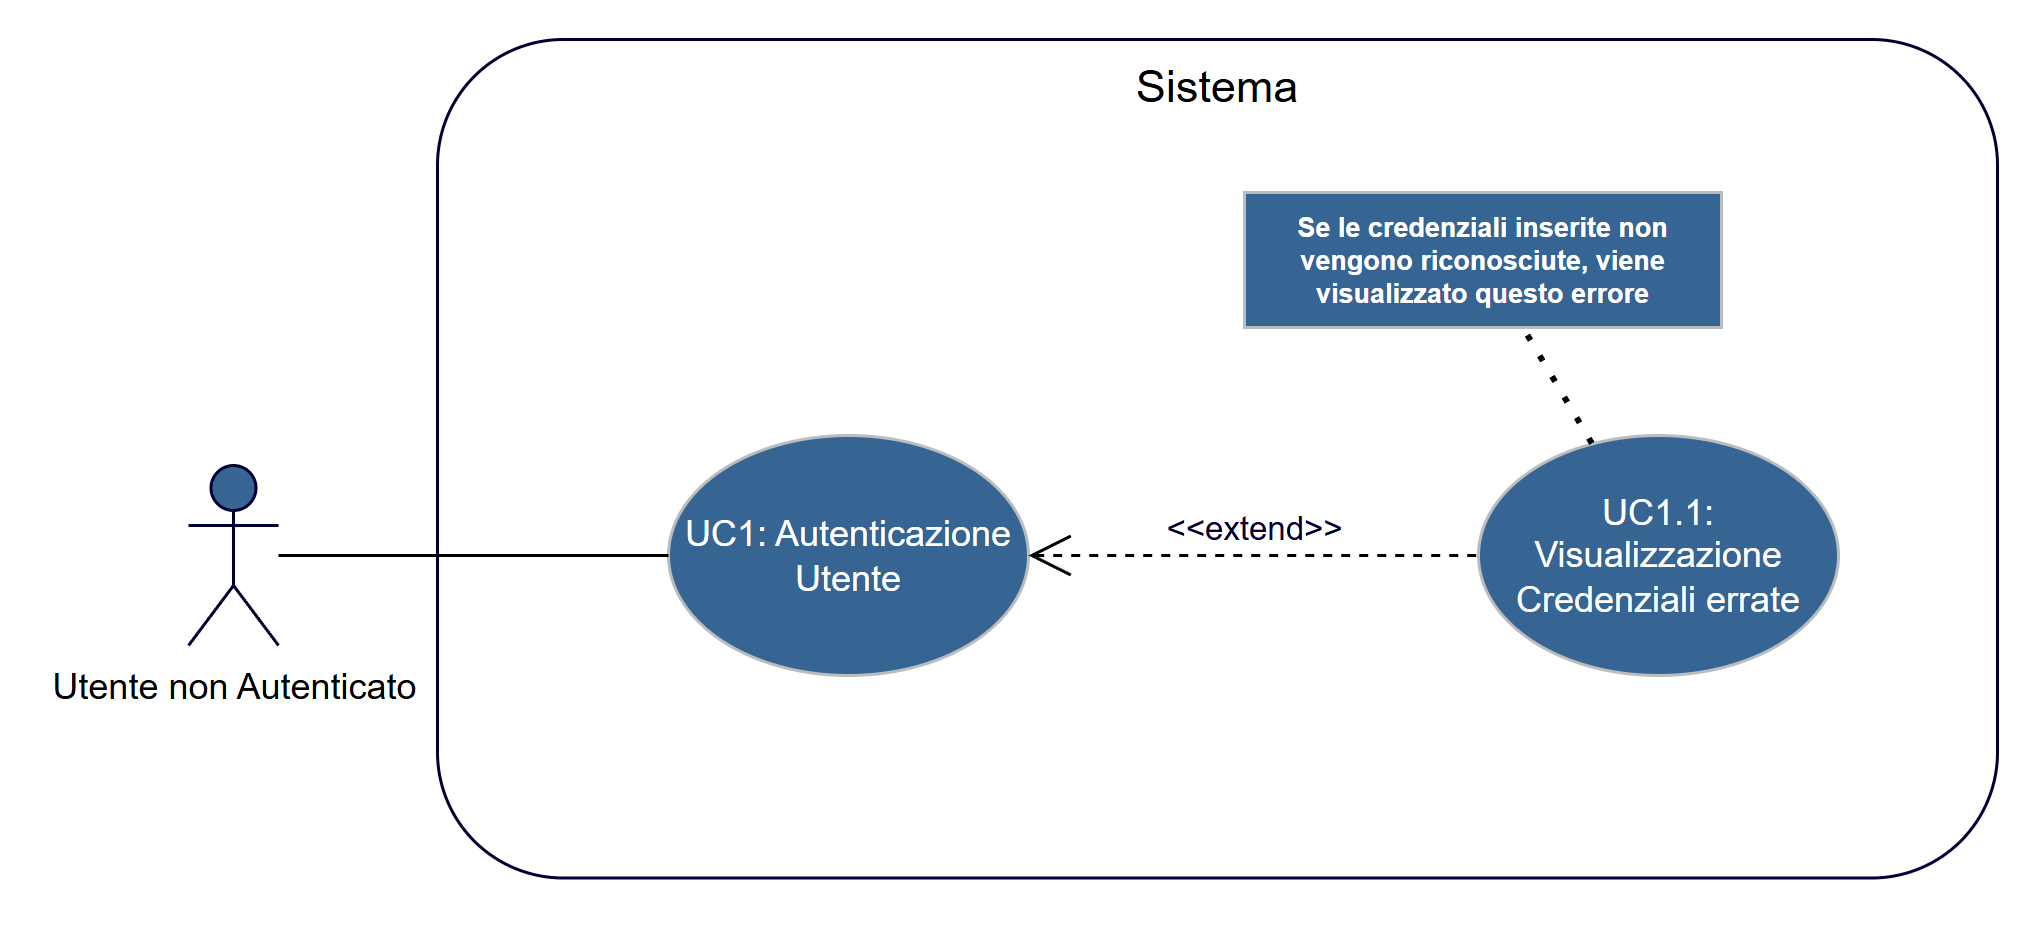
\includegraphics[alt={Diagramma UML Autenticazione Utente}, height=6cm]{img/usecase/UC1+UC1.1.png}
    \caption{UC1 + UC1.1.}
    \label{fig:uc1_login}
\end{figure}

\begin{usecase}{1}{Autenticazione Utente}
\usecaseactors{Utente non autenticato}
\usecasepre{L'utente si trova alla schermata di login.}
\usecasedesc{Il Sistema verifica le credenziali inserite e, se corrette, crea una sessione autenticata protetta.}
\usecasepost{L'utente accede alle funzionalità.}
\usecasealt{Se le credenziali non sono valide, viene mostrato un messaggio di errore (\hyperref[uc:uc1.1_errore_login]{UC1.1}).}
\label{uc:uc1_login}
\end{usecase}

\begin{usecase}{1.1}{Visualizzazione Credenziali Errate}
\usecaseactors{Utente non autenticato}
\usecasepre{L'utente si trova alla schermata di login.}
\usecasedesc{Il Sistema verifica le credenziali inserite e, se scorrette, mostra un messaggio di errore.}
\usecasepost{L'utente può riprovare reinserendo le credenziali.}
\label{uc:uc1.1_errore_login}
\end{usecase}

\newpage

\begin{figure}[htbp]
    \centering
    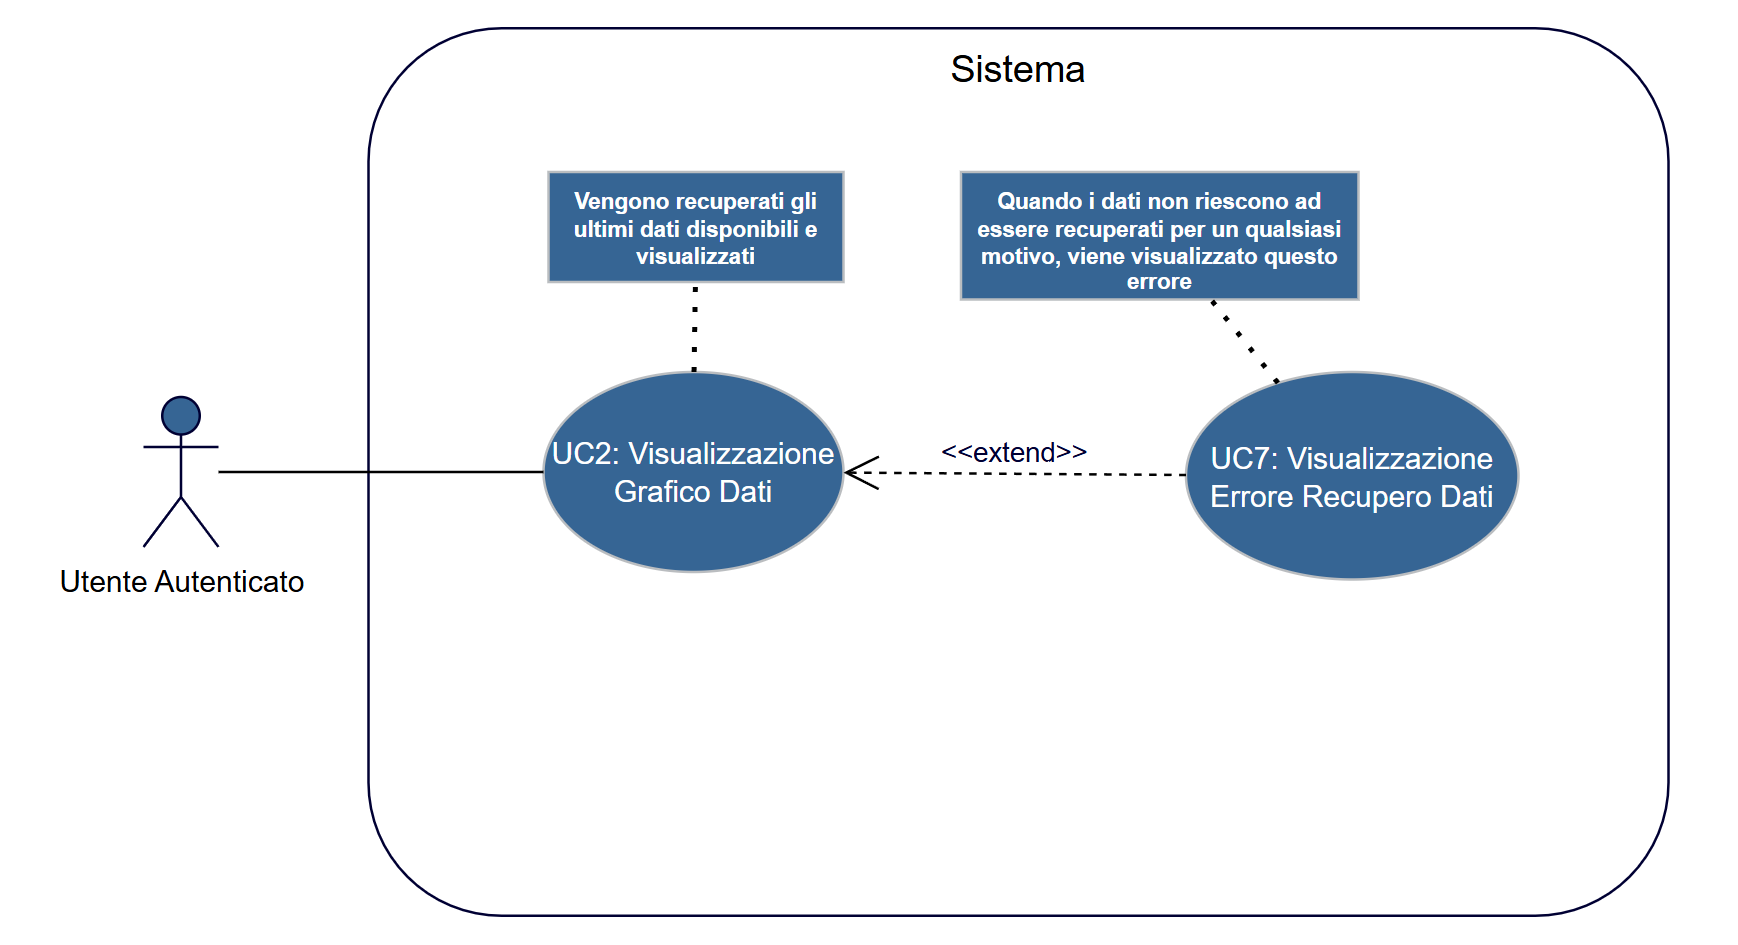
\includegraphics[alt={Diagramma UML Visualizzazione Grafico Dati}, height=7cm]{img/usecase/UC2+UC7.png}
    \caption{UC2 + UC7.}
    \label{fig:uc2_grafico}
\end{figure}

\begin{usecase}{2}{Visualizzazione Grafico Dati}
\usecaseactors{Utente}
\usecasepre{L'utente è autenticato.}
\usecasedesc{Il Sistema mostra un grafico con l'andamento temporale dei dati di produzione.}
\usecasepost{Il grafico viene aggiornato con l'ultima sincronizzazione disponibile.}
\usecasealt{Se i dati non sono presenti, viene visualizzato un messaggio di errore (\hyperref[uc:uc7_errore_dati]{UC7}).}
\label{uc:uc2_grafico}
\end{usecase}

\newpage

\begin{figure}[htbp]
    \centering
    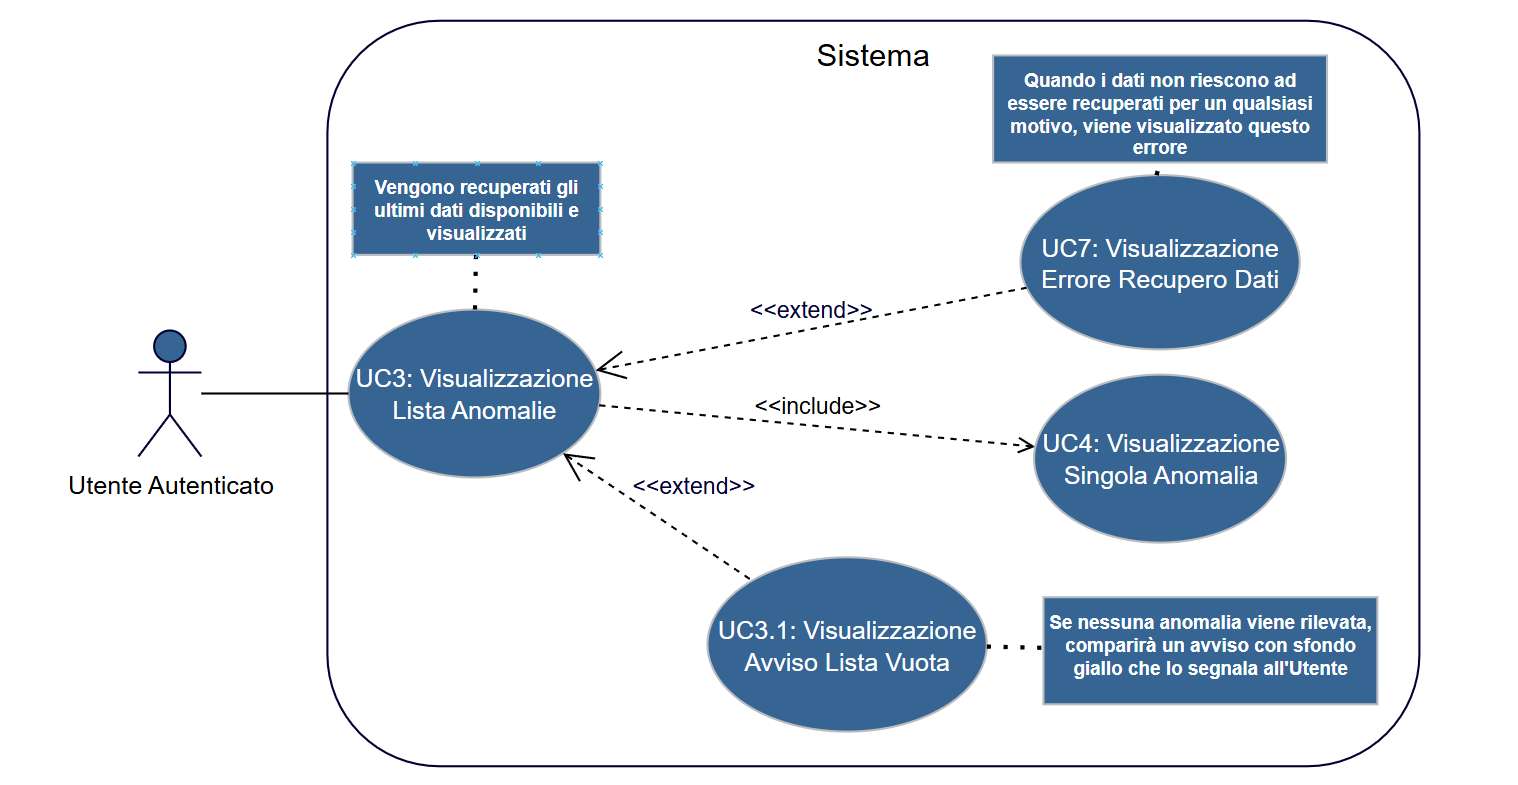
\includegraphics[alt={Diagramma UML Visualizzazione Lista Anomalie}, height=7cm]{img/usecase/UC3+UC4+UC7.png}
    \caption{UC3 + UC4 + UC7.}
    \label{fig:uc3_lista_anomalie}
\end{figure}

\begin{usecase}{3}{Visualizzazione Lista Anomalie}
\usecaseactors{Utente}
\usecasepre{Sono state eseguite analisi sui dati.}
\usecasedesc{Il Sistema elenca tutte le anomalie rilevate.}
\usecasepost{La lista è disponibile per ulteriori approfondimenti.}
\usecasealt{Se non esistono anomalie nel periodo selezionato, viene mostrato un messaggio informativo (\hyperref[uc:uc3.1_lista_anomalie_vuota]{UC3.1}).}
\usecasealt{Se il sistema non riesce a recuperare i dati, viene visualizzato un errore (\hyperref[uc:uc7_errore_dati]{UC7}).}
\label{uc:uc3_lista_anomalie}
\end{usecase}

\begin{usecase}{3.1}{Visualizzazione Avviso Lista Vuota}
\usecaseactors{Utente}
\usecasepre{Il Sistema notifica che non sono state rilevate anomalie.}
\usecasedesc{Viene visualizzato un avviso indicando l'assenza di anomalie.}
\label{uc:uc3.1_lista_anomalie_vuota}
\end{usecase}

\newpage

\begin{usecase}{4}{Dettaglio Anomalia}
\usecaseactors{Utente}
\usecasepre{L'utente ha selezionato una specifica anomalia dalla lista.}
\usecasedesc{Il Sistema visualizza grafici e \gls{log} di dettaglio relativi all'anomalia scelta.}
\usecasepost{L'utente può valutare la necessità di un intervento correttivo.}
\label{uc:uc4_dettaglio_anomalia}
\end{usecase}

\newpage

\begin{figure}[htbp]
    \centering
    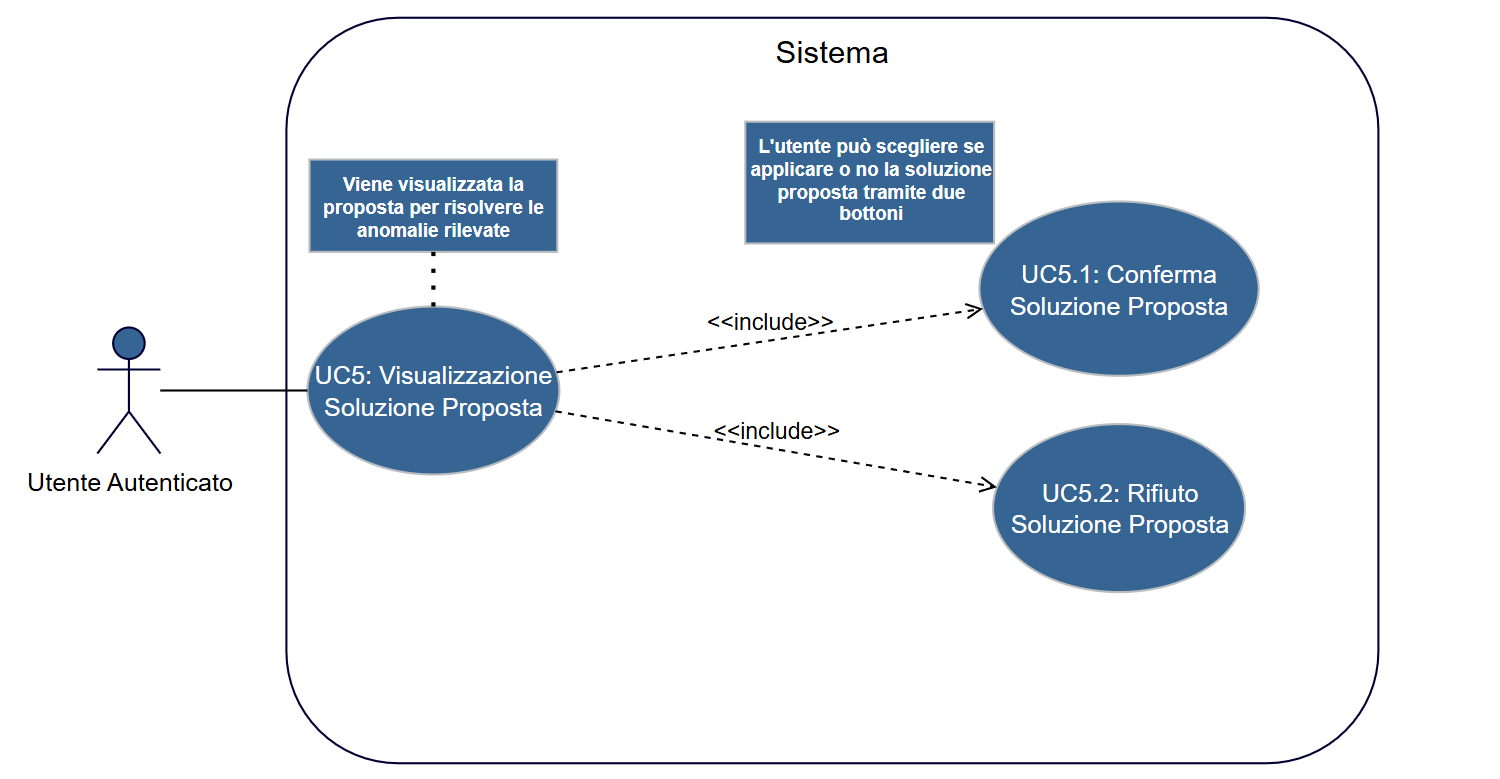
\includegraphics[alt={Diagramma UML Visualizzazione Soluzione Proposta}, height=7cm]{img/usecase/UC5+UC5.1+UC5.2.png}
    \caption{UC5 + UC5.1 + UC5.2.}
    \label{fig:uc5_soluzione_proposta}
\end{figure}

\begin{usecase}{5}{Visualizzazione Soluzione Proposta}
\usecaseactors{Utente}
\usecasepre{È stato selezionato un evento critico.}
\usecasedesc{Il Sistema visualizza una proposta di soluzione.}
\usecasepost{La soluzione può essere accettata (\hyperref[uc:uc5.2_conferma_soluzione]{UC5.2}) o ignorata (\hyperref[uc:uc5.1_rifiuto_soluzione]{UC5.1}).}
\label{uc:uc5_soluzione_proposta}
\end{usecase}

\begin{usecase}{5.1}{Rifiuto Soluzione Proposta}
\usecaseactors{Utente}
\usecasepre{È visualizzata una soluzione proposta (\hyperref[uc:uc5_soluzione_proposta]{UC5}).}
\usecasedesc{L'Utente rifiuta la soluzione proposta.}
\usecasepost{Il sistema registra il rifiuto e mantiene l'anomalia aperta.}
\label{uc:uc5.1_rifiuto_soluzione}
\end{usecase}

\newpage

\begin{usecase}{5.2}{Conferma Soluzione Proposta}
\usecaseactors{Utente}
\usecasepre{È visualizzata una soluzione proposta (\hyperref[uc:uc5_soluzione_proposta]{UC5}).}
\usecasedesc{L'Utente approva la soluzione che viene applicata al sistema di produzione.}
\usecasepost{Il sistema avvia l'esecuzione del piano correttivo.}
\label{uc:uc5.2_conferma_soluzione}
\end{usecase}

\newpage

\begin{figure}[htbp]
    \centering
    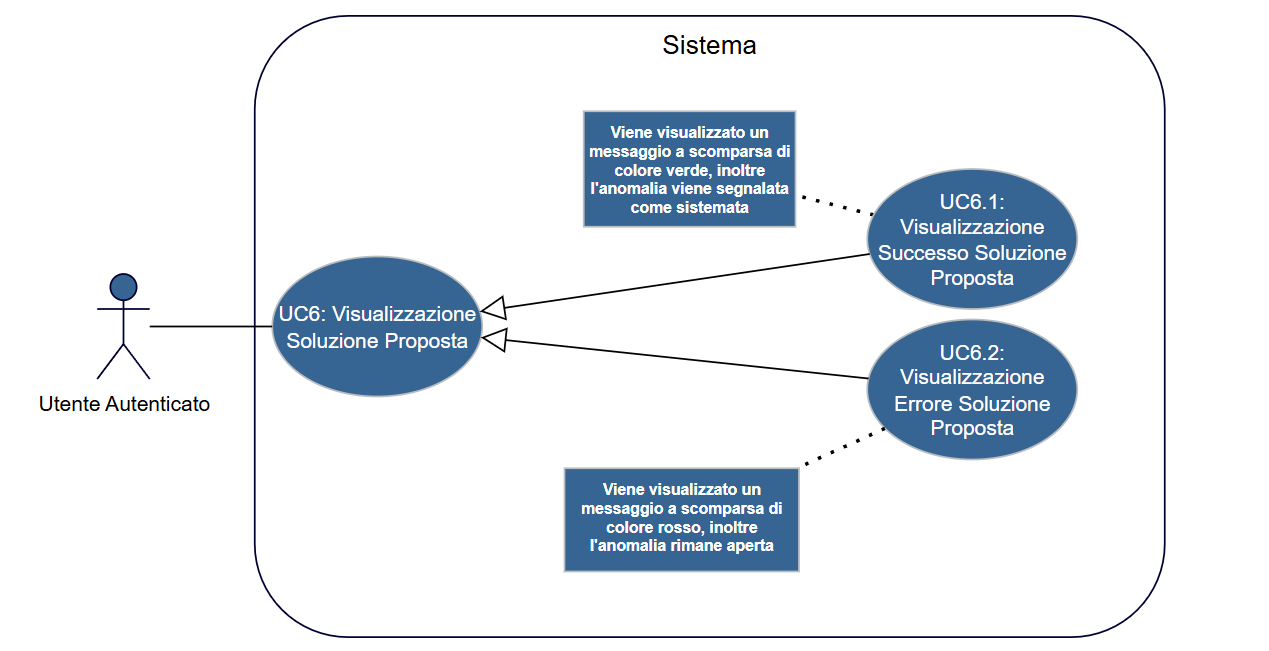
\includegraphics[alt={Diagramma UML Visualizzazione Soluzione Proposta}, height=7cm]{img/usecase/UC6+UC6.1+UC6.2.png}
    \caption{UC6 + UC6.1 + UC6.2.}
    \label{fig:uc6_visualizzazione_soluzione}
\end{figure}

\begin{usecase}{6}{Visualizzazione Risultato Soluzione Proposta}
\usecaseactors{Utente}
\usecasepre{Il piano correttivo è stato approvato ed eseguito.}
\usecasedesc{Il Sistema notifica all'Utente il risultato.}
\usecasepost{In base all’esito dell’applicazione, il messaggio può essere positivo (\hyperref[uc:uc6.1_soluzione_ok]{UC6.1}) o negativo (\hyperref[uc:uc6.2_soluzione_err]{UC6.2}).}
\label{uc:uc6_visualizzazione_soluzione}
\end{usecase}

\begin{usecase}{6.1}{Visualizzazione Successo Soluzione Proposta}
\usecaseactors{Utente}
\usecasepre{Il piano correttivo è stato eseguito correttamente.}
\usecasedesc{Il Sistema notifica all'Utente l'avvenuta applicazione della soluzione.}
\usecasepost{L'anomalia viene marcata come risolta.}
\label{uc:uc6.1_soluzione_ok}
\end{usecase}

\newpage

\begin{usecase}{6.2}{Visualizzazione Errore Soluzione Proposta}
\usecaseactors{Utente}
\usecasepre{Il sistema ha tentato di applicare una soluzione proposta.}
\usecasedesc{Il Sistema segnala all'Utente il fallimento dell'applicazione e fornisce i dettagli dell'errore.}
\usecasepost{L'anomalia resta aperta e viene registrato il tentativo fallito.}
\label{uc:uc6.2_soluzione_err}
\end{usecase}

\begin{usecase}{7}{Visualizzazione Errore Recupero Dati}
\usecaseactors{Utente}
\usecasepre{L'utente è autenticato.}
\usecasedesc{Il Sistema mostra un errore perché i dati non sono presenti.}
\usecasepost{L'Utente può aggiornare la pagina per riprovare a recuperare i dati.}
\label{uc:uc7_errore_dati}
\end{usecase}

\newpage

%--------------------------------------------------------------------------
% Casi d'uso desiderabili
%--------------------------------------------------------------------------
\subsection{Casi d'uso desiderabili}
I seguenti casi d'uso rappresentano le funzionalità desiderabili che il sistema potrebbe implementare per migliorare l'esperienza dell'utente e fornire funzionalità aggiuntive.

\begin{figure}[htbp]
    \centering
    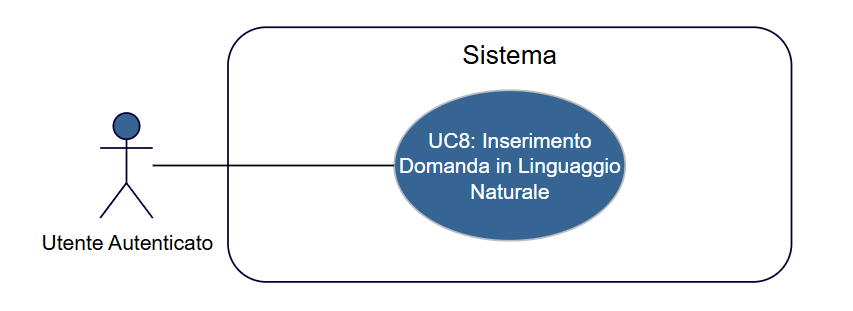
\includegraphics[alt={Diagramma UML Inserimento Domanda in Linguaggio Naturale}, height=5cm]{img/usecase/UC8.png}
    \caption{UC8.}
    \label{fig:uc8_domanda_nl}
\end{figure}

\begin{usecase}{8}{Inserimento Domanda in Linguaggio Naturale}
\usecaseactors{Utente}
\usecasepre{L'utente è autenticato.}
\usecasedesc{L'utente inserisce una domanda libera relativa al sistema.}
\usecasepost{La domanda viene inoltrata al \gls{LLM}.}
\label{uc:uc8_domanda_nl}
\end{usecase}

\newpage

\begin{figure}[htbp]
    \centering
    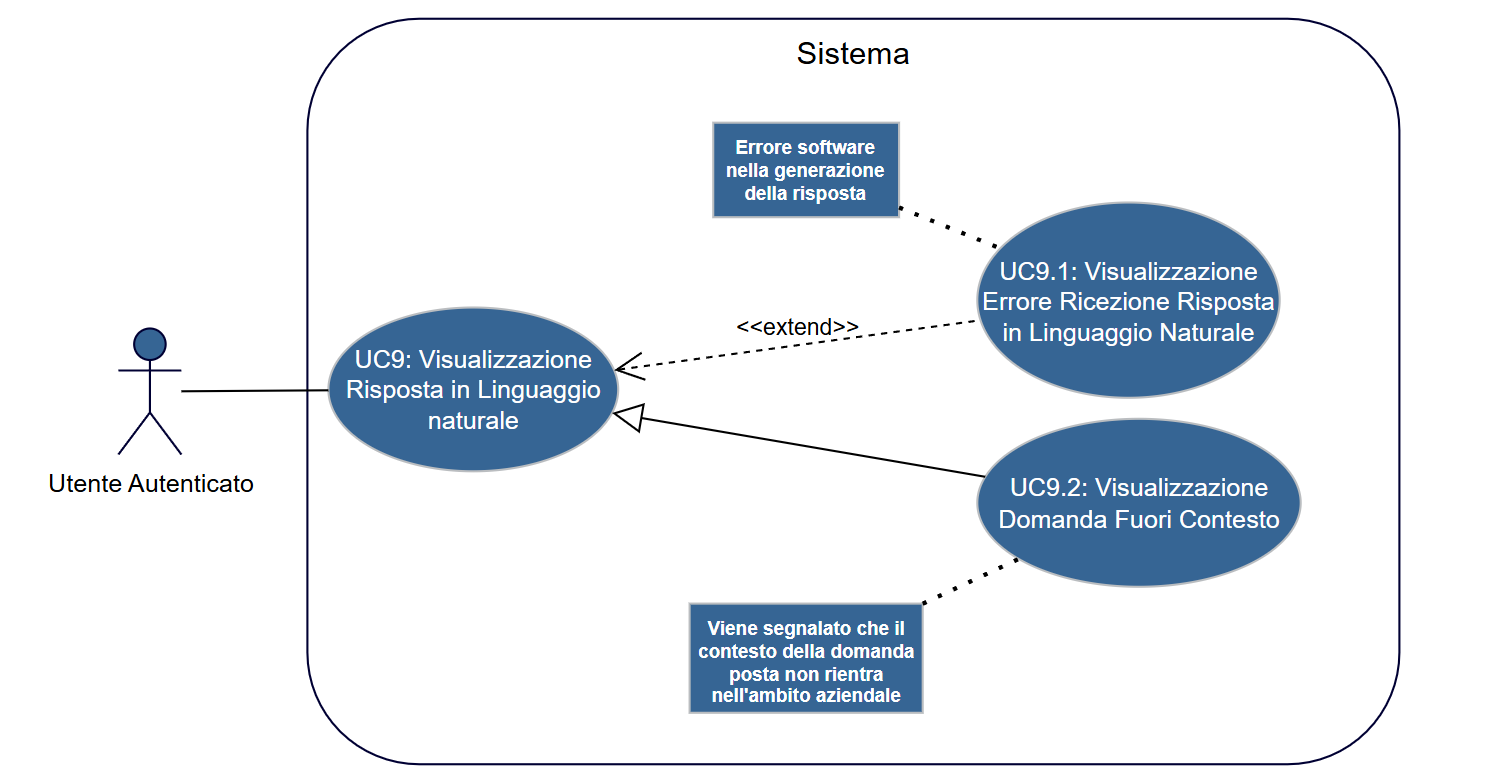
\includegraphics[alt={Diagramma UML Visualizzazione Risposta in Linguaggio Naturale}, height=7cm]{img/usecase/UC9+UC9.1+UC9.2.png}
    \caption{UC9 + UC9.1 + UC9.2.}
    \label{fig:uc9_risposta_nl}
\end{figure}

\begin{usecase}{9}{Visualizzazione Risposta in Linguaggio Naturale}
\usecaseactors{Utente}
\usecasepre{È stata inoltrata una domanda (\hyperref[uc:uc8_domanda_nl]{UC8}).}
\usecasedesc{Viene visualizzata una risposta generata in linguaggio naturale.}
\usecasepost{La risposta è visualizzata all'Utente.}
\usecasealt{Se si verifica un errore, viene mostrato un messaggio di errore (\hyperref[uc:uc9.1_errore_nl]{UC9.1}).}
\usecasealt{Se la domanda è fuori contesto, il Sistema chiede all'utente di riformulare (\hyperref[uc:uc9.2_fuori_contesto_nl]{UC9.2}).}
\label{uc:uc9_risposta_nl}
\end{usecase}

\begin{usecase}{9.1}{Visualizzazione Errore Ricezione Risposta in Linguaggio Naturale}
\usecaseactors{Utente}
\usecasepre{È stata inoltrata una domanda (\hyperref[uc:uc8_domanda_nl]{UC8}).}
\usecasedesc{Il sistema non riesce a recuperare la risposta.}
\usecasepost{L'utente visualizza un errore che lo informa del problema.}
\label{uc:uc9.1_errore_nl}
\end{usecase}

\newpage

\begin{usecase}{9.2}{Visualizzazione domanda fuori contesto}
\usecaseactors{Utente}
\usecasepre{È stata inoltrata una domanda (\hyperref[uc:uc8_domanda_nl]{UC8}) non inerente all'ambito operativo.}
\usecasedesc{L'utente visualizza un avviso che la domanda posta era fuori contesto.}
\usecasepost{L'utente può riformulare la domanda.}
\label{uc:uc9.2_fuori_contesto_nl}
\end{usecase}

\newpage

\begin{figure}[htbp]
    \centering
    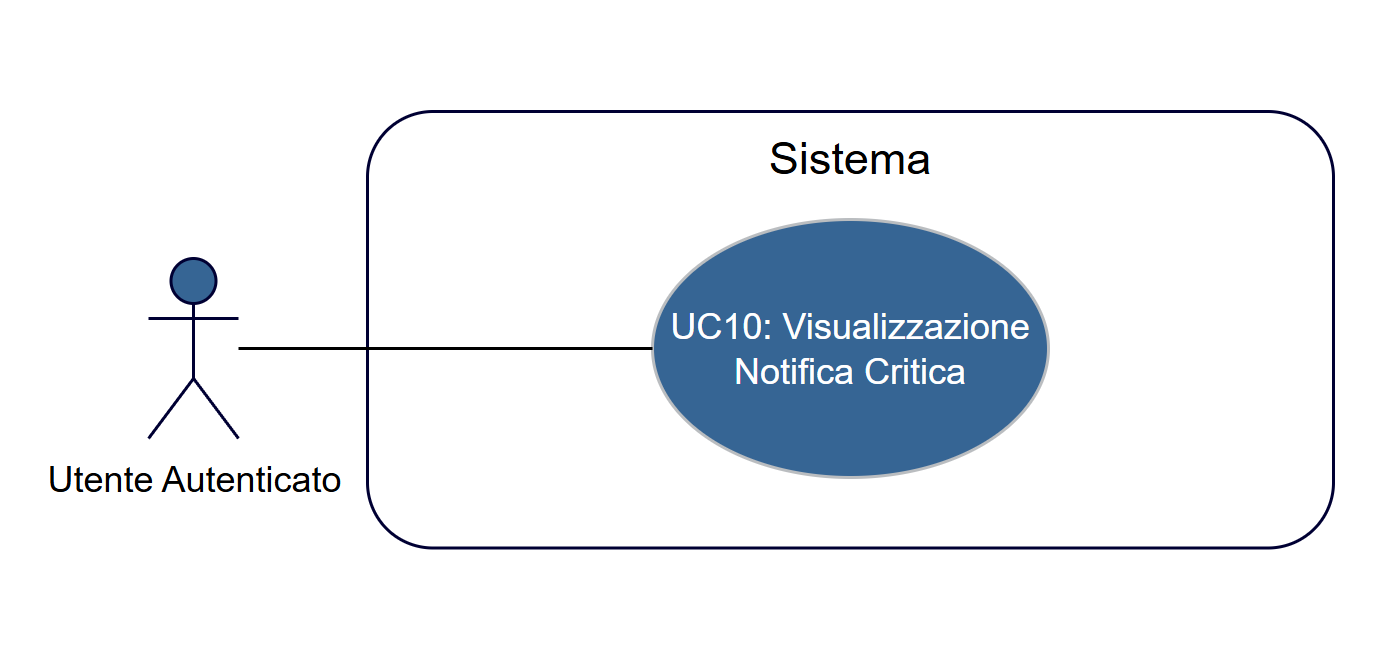
\includegraphics[alt={Diagramma UML Visualizzazione Notifica Critica}, height=5cm]{img/usecase/UC10.png}
    \caption{UC10.}
    \label{fig:uc10_notifiche}
\end{figure}


\begin{usecase}{10}{Visualizzazione Notifica Critica}
\usecaseactors{Utente}
\usecasepre{Il sistema rileva un'anomalia critica.}
\usecasedesc{Viene visualizzato un avviso sui dispositivi connessi.}
\usecasepost{Gli operatori visualizzano l'avviso.}
\label{uc:uc10_notifiche}
\end{usecase}

%--------------------------------------------------------------------------
% Casi d'uso facoltativi
%--------------------------------------------------------------------------

\newpage

\subsection{Casi d'uso facoltativi}
I seguenti casi d'uso rappresentano le funzionalità facoltative che il sistema potrebbe implementare per migliorare l'esperienza dell'utente e fornire funzionalità aggiuntive.

\begin{figure}[htbp]
    \centering
    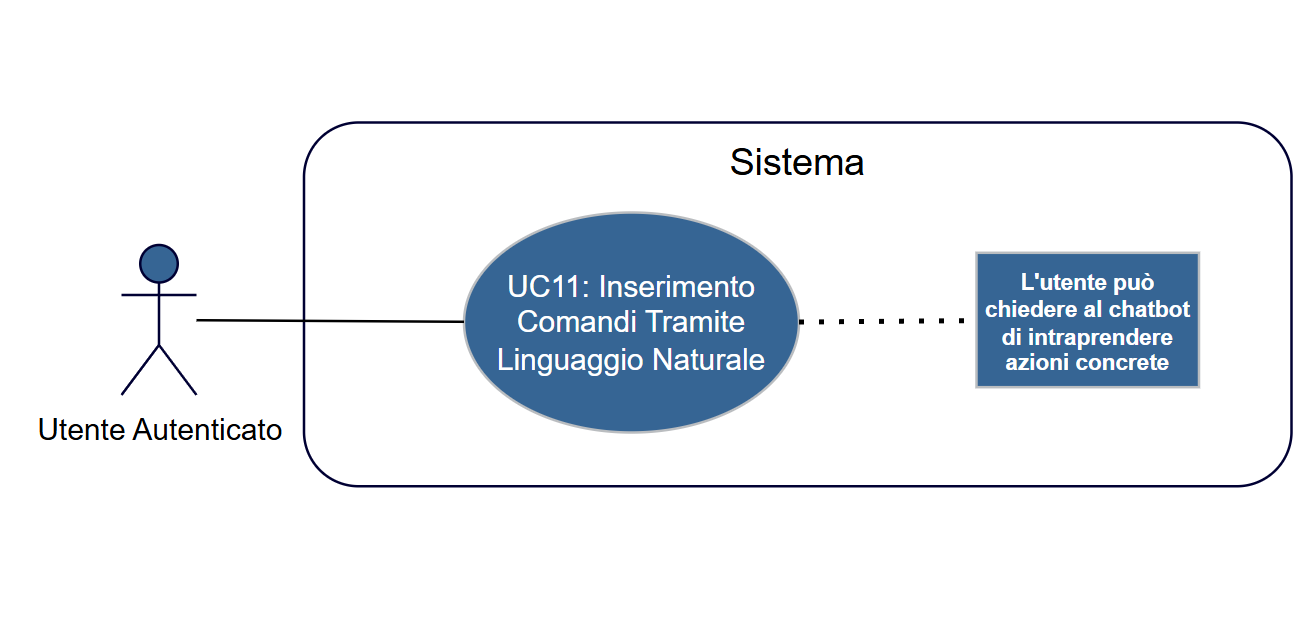
\includegraphics[alt={Diagramma UML Inserimento Comandi Tramite Linguaggio Naturale}, height=5cm]{img/usecase/UC11.png}
    \caption{UC11.}
    \label{fig:uc11_comandi_nl}
\end{figure}

\begin{usecase}{11}{Inserimento Comandi Tramite Linguaggio Naturale}
\usecaseactors{Utente}
\usecasepre{L'utente è autenticato e l'interfaccia chat è attiva.}
\usecasedesc{L'utente impartisce comandi operativi in linguaggio naturale; il Sistema li interpreta e li esegue.}
\usecasepost{L'azione richiesta viene completata o ne viene comunicato l'esito.}
\label{uc:uc11_comandi_nl}
\end{usecase}

\newpage

%--------------------------------------------------------------------------
% Tracciamento dei requisiti
%--------------------------------------------------------------------------
\section{Tracciamento dei requisiti}
Il tracciamento mostra la copertura dei requisiti funzionali (F) classificati come
\textbf{N} (obbligatori), \textbf{D} (desiderabili) e \textbf{Z} (facoltativi).

\begin{center}
  \brandTableColors
  \begin{longtable}{|p{2.25cm}|p{7.75cm}|p{2.25cm}|}
    \hline
    \multicolumn{1}{|c|}{\textbf{Requisito}} &
    \multicolumn{1}{c|}{\textbf{Descrizione}} &
    \multicolumn{1}{c|}{\textbf{Use Case}}\\
    \hline
    FN1 & Login sicuro dell'utente                                    & UC1, UC1.1 \\ \hline
    FN2 & Visualizzare grafico dei dati di produzione                 & UC2, UC7   \\ \hline
    FN3 & \textit{Dashboard} anomalie rilevate                               & UC3, UC3.1, UC7, UC4 \\ \hline
    FN4 & Presentare una soluzione proposta tramite LLM               & UC5, UC5.1, UC5.2 \\ \hline
    FN5 & Gestire l'accettazione/rifiuto di una soluzione             & UC5.1, UC5.2 \\ \hline
    FN6 & Notificare risultato applicazione soluzione                 & UC6, UC6.1, UC6.2 \\ \hline
    FN7 & Gestire errori di recupero dati                             & UC7        \\ \hline
    FD1 & Inserire domande in linguaggio naturale                     & UC8        \\ \hline
    FD2 & Ricevere risposte in linguaggio naturale                    & UC9, UC9.1, UC9.2 \\ \hline
    FD3 & Visualizzare notifiche critiche                             & UC10       \\ \hline
    FZ1 & Inserire comandi in linguaggio naturale                     & UC11       \\ \hline
  \end{longtable}
  \captionof{table}{Tracciamento dei requisiti funzionali.}
  \label{tab:requisiti_fun}
\end{center}

